\documentclass[11pt]{article}
\usepackage[a4paper,margin=24mm]{geometry}
\usepackage{amsmath,amssymb,booktabs,graphicx,xcolor,hyperref,fancyhdr,lmodern}
\definecolor{ink}{HTML}{173853}
\hypersetup{colorlinks=true,linkcolor=ink,urlcolor=ink}
\pagestyle{fancy}\fancyhf{}\lhead{\small\textcolor{ink}{MAX-CUT / ROUNDING METHODS}}\rhead{\small Hyperplane sweep}\cfoot{\thepage}\setlength{\headheight}{14pt}
\setlength{\parindent}{0pt}\setlength{\parskip}{5pt}
\newcommand{\R}{\mathbb R}\newcommand{\sgn}{\operatorname{sgn}_{-}}
\newcommand{\sect}[1]{\section*{\textcolor{ink}{#1}}}
\newcommand{\figcap}[1]{{\small\textit{#1}}}
\begin{document}
{\color{ink}\LARGE\bfseries Hyperplane Sweep}\par
{\large From random GW rounding to event-driven optimization}\par
\smallskip
\textbf{Idea.} Keep the embedded graph vertices fixed. Rotate the separating hyperplane, find the best cut along the rotation, and repeat from the best direction. No new SDP solve or clustering is required.

\sect{1. Start from the EVA embedding}
Let $G=(V,E,w)$ be an undirected graph with $n$ vertices, $m$ edges and original weights $w_{ij}$ (possibly negative). The EVA solver provides a factor
\[
Y=\begin{pmatrix}y_1^\top\\ \vdots\\ y_n^\top\end{pmatrix}\in\R^{n\times p},\qquad X=YY^\top,\qquad \|y_i\|_2=1.
\]
Each row is a vertex embedded in $p$ dimensions. Throughout the algorithm, $Y$ remains fixed. Goemans--Williamson (GW) rounding samples a unit normal $r\in\mathbb S^{p-1}$ and uses the hyperplane
\[
H(r)=\{y\in\R^p:y^\top r=0\},\qquad
x_i(r)=\sgn(y_i^\top r)=\begin{cases}+1,&y_i^\top r>0,\\-1,&y_i^\top r\leq0.\end{cases}
\]
Here $\mathbb S^{p-1}=\{r\in\R^p:\|r\|_2=1\}$. The goal is to maximize the original cut, not a clustering objective:
\[
F(r)=C(x(r)),\qquad C(x)=\frac12\sum_{\{i,j\}\in E}w_{ij}(1-x_ix_j)=\frac14x^\top Lx.
\]
The weighted graph Laplacian is $L=D-W$, with symmetric weight matrix $W$ and $D_{ii}=\sum_j w_{ij}$.

\sect{2. The idea in two dimensions}
In $\R^2$, the separating hyperplane is a line through the origin. A small rotation often leaves every vertex on its original side. The cut changes only when the line crosses an embedded vertex.
\begin{center}
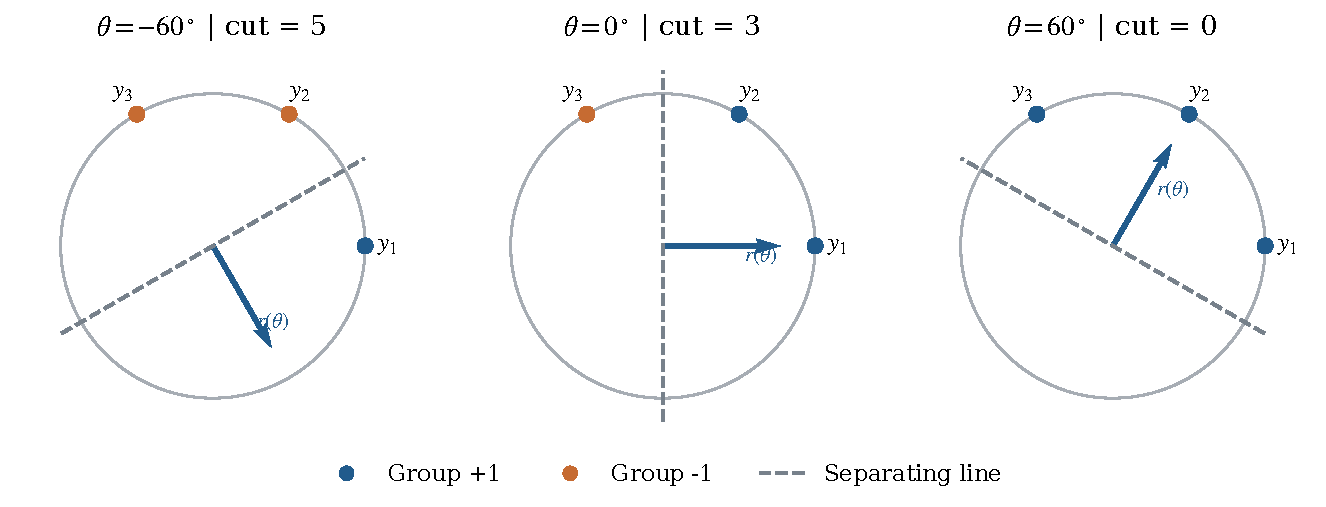
\includegraphics[width=\linewidth]{r2.pdf}\par
\figcap{Figure 1. The same three embedded vectors at three angles. Edge weights are $w_{12}=3$, $w_{13}=2$, $w_{23}=1$.}
\end{center}
\newpage
\sect{3. The mathematics of one rotation}
Take two orthogonal unit vectors $r,u\in\R^p$: $r^\top u=0$. The vector $u$ defines the direction of rotation and their span defines a two-dimensional plane.
\begin{equation}
\boxed{r(\theta)=r\cos\theta+u\sin\theta},\qquad -\pi/2<\theta<\pi/2.
\end{equation}
The vector remains on the unit sphere because
\[
\|r(\theta)\|^2=\cos^2\theta+\sin^2\theta+2r^\top u\cos\theta\sin\theta=1.
\]
The initial GW direction corresponds to $\theta=0$. A semicircle suffices for generic, event-free partitions in this plane, up to group exchange, because opposite normals give the same cut away from ties.

\textbf{Find the crossing angles analytically.} Define $a_i=y_i^\top r$ and $b_i=y_i^\top u$. Then
\[
x_i(\theta)=\sgn(a_i\cos\theta+b_i\sin\theta).
\]
A sign change occurs at a zero. On the open semicircle $\cos\theta>0$, so for $b_i\ne0$,
\begin{align*}
a_i\cos\theta+b_i\sin\theta&=0,\\
a_i+b_i\tan\theta&=0,\\
\boxed{\theta_i=\arctan(-a_i/b_i).}&
\end{align*}
Every such vertex has one crossing. When $b_i=0$, its sign is constant on the open interval; when $a_i=b_i=0$, it always receives $-1$ under this convention. Sort distinct crossing angles. Between consecutive events the partition is constant; only one representative per interval is needed.

\textbf{Worked example.} In Figure 1, $r=(1,0)^\top$, $u=(0,1)^\top$, and the rows of $Y$ point at $0^\circ,60^\circ,120^\circ$. Vertex 1 never crosses inside the arc; vertices 2 and 3 cross at $-30^\circ$ and $30^\circ$.
\begin{center}
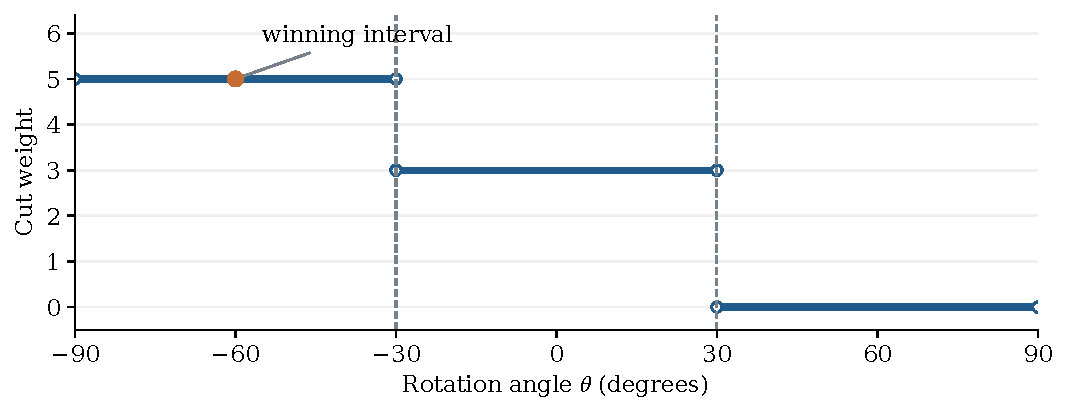
\includegraphics[width=.82\linewidth]{events.pdf}\par
\figcap{Figure 2. Actual cut values for Figure 1. The starting GW cut is 3; the winning interval has cut 5. Open endpoints exclude event-angle ties.}
\end{center}
The midpoint of the winning interval $(-90^\circ,-30^\circ)$ is $-60^\circ$, giving $r^*=(1/2,-\sqrt{3}/2)^\top$.
\newpage
\sect{4. From two to three dimensions}
In $\R^2$, a fixed unit vector $r$ has only two perpendicular unit vectors, $u$ and $-u$. Both specify the same rotation plane. In $\R^3$, the perpendicular vectors form a two-dimensional plane, with infinitely many perpendicular unit vectors. Each choice of $u$ defines a great-circle path for the normal.
\begin{center}
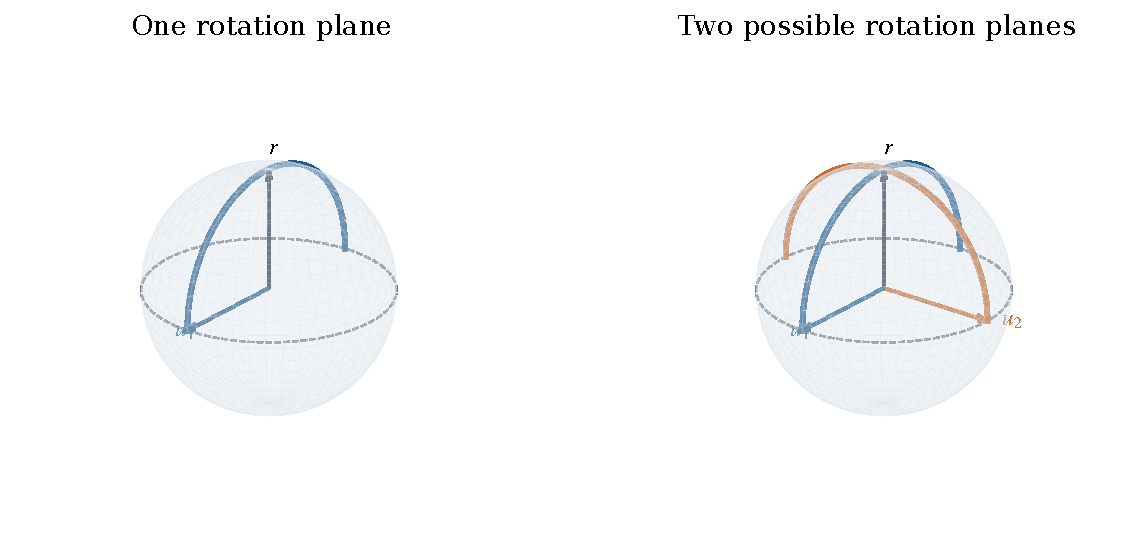
\includegraphics[width=\linewidth]{r3.pdf}\par
\figcap{Figure 3. The sphere represents possible unit normals. The equator is the set of perpendicular unit vectors for the initial normal $r$. Different choices of $u$ produce different paths.}
\end{center}
The separating hyperplane has dimension $p-1$; the rotation plane $\operatorname{span}\{r,u\}$ always has dimension two. They are different objects.

\sect{5. Generating a rotation in higher dimensions}
In $\R^p$, the perpendicular subspace $r^\perp=\{u:r^\top u=0\}$ has dimension $p-1$. If the EVA factor has $p=119$ columns, there are 118 linearly independent perpendicular directions and infinitely many perpendicular unit vectors. We need only one per sweep.
Sample $z\sim\mathcal N(0,I_p)$. Since $r$ is a unit vector, its parallel component is $(z^\top r)r$. Subtract this component and normalize:
\begin{equation}
\boxed{h=z-(z^\top r)r,\qquad u=h/\|h\|}.
\end{equation}
This is one Gram--Schmidt orthogonalization step. Indeed,
\[
r^\top h=r^\top z-(z^\top r)\underbrace{r^\top r}_{1}=0.
\]
Normalization preserves orthogonality. If the residual is zero or numerically too small, draw again. The pair $(r,u)$ defines a two-dimensional search plane even in hundreds of dimensions. After an improvement, sample the next tangent relative to the new normal.
\newpage
\sect{6. Efficiently evaluate the cut at each event}
Only edges incident to a vertex can change their contribution when its spin flips. Let $x'$ be obtained by flipping $x_i$ to $-x_i$. The improvement is
\begin{align*}
\Delta_i&=C(x')-C(x)\\
&=\frac12\sum_{j\in N(i)}w_{ij}\big[(1+x_ix_j)-(1-x_ix_j)\big]\\
&=\boxed{x_i\sum_{j\in N(i)}w_{ij}x_j}.
\end{align*}
A positive gain improves the cut; a negative gain worsens it. The formula works with negative weights.

\textbf{Maintain the flip gains.} Initialize $\Delta=x\odot(Wx)$, where $\odot$ denotes elementwise multiplication. At a crossing of $i$, save $s=x_i$ and $d=\Delta_i$. Update
\begin{align*}
C&\leftarrow C+d,\\
\Delta_j&\leftarrow\Delta_j-2w_{ij}s x_j,\qquad j\in N(i),\\
x_i&\leftarrow-s,\qquad\Delta_i\leftarrow-d.
\end{align*}
The neighbor update follows because the term $w_{ij}x_jx_i$ changes sign. Nonincident gains stay unchanged. When multiple vertices share an event angle, flip them sequentially but compare the cut only after the whole group flips; intermediate partitions may not be realizable on an open interval.

\textbf{Example.} In Figure 2 the first interval has $x=(+1,-1,-1)$ and $C=5$. At $-30^\circ$, vertex 2 flips, with
\[
\Delta_2=(-1)[3(+1)+1(-1)]=-2.
\]
The new cut is $3$. At $30^\circ$, vertex 3 flips with gain $(-1)[2(+1)+1(+1)]=-3$, giving cut zero. Keep the first interval, not the final one.

\textbf{Cost of one sweep.} Each vertex crosses at most once. With adjacency lists all gain updates visit each edge at most twice.
\begin{center}
\begin{tabular}{@{}lr@{}}\toprule
Operation & Complexity\\\midrule
Compute $a=Yr$, $b=Yu$ & $O(np)$\\
Sort crossing angles & $O(n\log n)$\\
Initial cut, gains and incremental updates & $O(n+m)$\\
Reconstruct and independently rescore winner & $O(np+m)$\\\bottomrule
\end{tabular}
\end{center}
The total is $O(np+n\log n+m)$. Store the winning interval rather than copying the entire partition at every improvement.
\newpage
\sect{7. Pseudocode: one exact event sweep}
\textbf{Inputs:} $Y,G$, unit normal $r$, unit tangent $u\perp r$. \textbf{Output:} a normal and its realized cut.
\begingroup\small
\begin{tabular}{@{}r p{.88\linewidth}@{}}
1 & Compute $a=Yr$, $b=Yu$. For $b_i\ne0$, form event $(\arctan(-a_i/b_i),i)$.\\
2 & Sort events by angle, grouping equal angles; add boundaries $-\pi/2,\pi/2$.\\
3 & Initialize $x$ at the first open interval midpoint. Compute $C(x)$ and $\Delta=x\odot(Wx)$. Record this interval as best.\\
4 & \textbf{For each} event group in increasing angular order:\\
5 & \quad\textbf{For each} vertex $i$ in the group: save $s=x_i$ and $d=\Delta_i$.\\
6 & \qquad $C\leftarrow C+d$; for each neighbor $j$, set $\Delta_j\leftarrow\Delta_j-2w_{ij}s x_j$.\\
7 & \qquad $x_i\leftarrow-s$; $\Delta_i\leftarrow-d$.\\
8 & \quad\textbf{If} $C$ exceeds the best score, save the next interval and score.\\
9 & Let $\theta^*$ be the winning midpoint. Compute $q=r\cos\theta^*+u\sin\theta^*$.\\
10 & Independently reconstruct and score the cut from $q$. Return $q$ if valid and no worse than $r$; otherwise return $r$.\\
\end{tabular}
\endgroup

\sect{8. Pseudocode: repeated hyperplane sweeps}
\textbf{Inputs:} $Y,G$, sweep budget $T$, optional initial GW normal. \textbf{Output:} best normal, partition and cut.
\begingroup\small
\begin{tabular}{@{}r p{.88\linewidth}@{}}
1 & Initialize $r=z_0/\|z_0\|$, $z_0\sim\mathcal N(0,I_p)$, or use a supplied GW normal. Set $B=F(r)$.\\
2 & \textbf{For} $t=1,\ldots,T$:\\
3 & \quad Sample $z\sim\mathcal N(0,I_p)$; compute $h=z-(z^\top r)r$.\\
4 & \quad If $\|h\|$ is too small, resample; otherwise set $u=h/\|h\|$.\\
5 & \quad $q\leftarrow\textsc{Sweep}(G,Y,r,u)$.\\
6 & \quad \textbf{If} $F(q)>B$, set $r\leftarrow q$, $B\leftarrow F(q)$.\\
7 & \textbf{Return} $r$, $x(r)$ and $B$.\\
\end{tabular}
\endgroup

\sect{9. What is guaranteed?}
The incumbent never worsens: $F(r_0)\le F(r_1)\le\cdots\le F(r_T)$. One sweep is exact over event-free intervals on its chosen arc in exact arithmetic. This is not a global optimum guarantee. Degenerate ties and floating-point reconstruction require verification; the fallback preserves the starting cut. Later discrete Flip/KL/ILS refinement is separate and may leave the family of hyperplane cuts. The random-tangent pseudocode is the core method; the research implementation explores guided proposals as well.
\newpage
\sect{10. A worked example in three dimensions}
The companion dashboard uses eight fixed unit vectors and 13 signed weighted edges. It begins with $r=(0,0,1)^\top$ and $z=(0.9,0.6,0.8)^\top$. Gram--Schmidt gives
\[
(z^\top r)r=(0,0,0.8)^\top,\quad h=(0.9,0.6,0)^\top,\quad
u=(0.9,0.6,0)^\top/\sqrt{1.17}.
\]
The rotation plane is $P=\operatorname{span}\{r,u\}$. The separating plane is $H(\theta)=\{y:y^\top r(\theta)=0\}$. The former stays fixed during one sweep; the latter rotates. The best interval is approximately $(-70.31^\circ,-32.66^\circ)$, with midpoint $\theta^*\approx-51.48^\circ$. The cut improves from 14 to 23.
\begin{center}
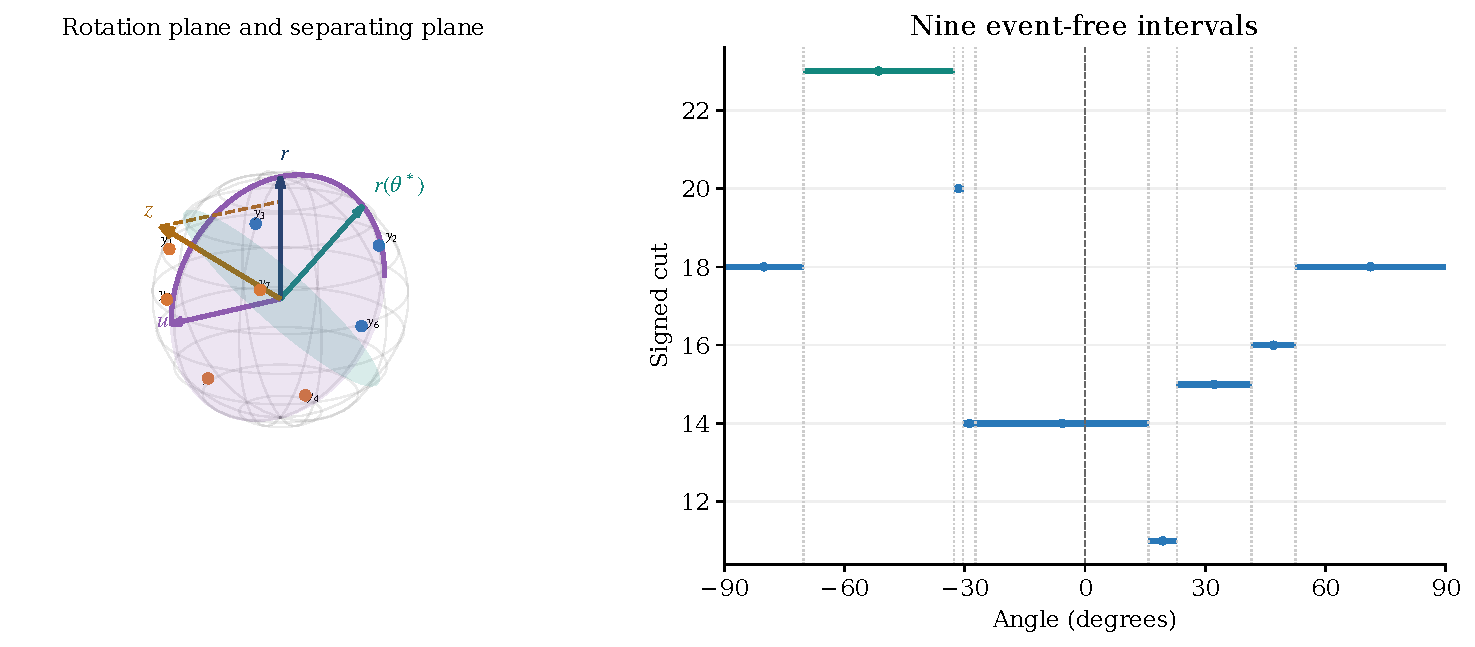
\includegraphics[width=\linewidth]{worked_r3.pdf}\par
\figcap{Figure 4. The lavender rotation plane contains the normal; the green separating plane divides the vertices. The right panel plots actual signed cut values between crossing angles.}
\end{center}
\textbf{Try it.} Open the \href{https://heri-espino.github.io/maxkcut/dashboard/}{companion dashboard}. Change $z$, move the angle slider, select the best interval and accept the improved normal. The next sweep chooses a new tangent. The demo evaluates interval cuts directly; Section 6 derives incremental updates.

\sect{11. Tangent proposals in the research implementation}
The same sweep can use different proposals, all projected onto $r^\perp$ and normalized.
\begin{center}\small
\begin{tabular}{@{}p{.22\linewidth}p{.71\linewidth}@{}}\toprule
Mode & Proposal before orthogonalization\\\midrule
Random & $z\sim\mathcal N(0,I_p)$.\\
Gain-guided & $z=\sum_{i\in S}(-x_i)(-\Delta_i)y_i$, where $S=\{i:\Delta_i<-10^{-9}\}$; falls back to boundary mode if empty.\\
Boundary-guided & $z=\sum_{i\in S}\varepsilon_i y_i$ with independent random signs; $S$ contains up to 96 vertices with smallest $|\Delta_i|$.\\\bottomrule
\end{tabular}
\end{center}
\textbf{Caution.} Negative flip gains are harmful flips, not improving ones. Small absolute gains are not necessarily small geometric margins $|y_i^\top r|$. These are exploratory heuristics; the acceptance check is unchanged. The dashboard demonstrates the random-tangent mode.
\end{document}
